\documentclass{article}
\usepackage{graphicx} % Required for inserting images
\usepackage{minted}

\title{Monte Carlo Techniques}
\author{Alex Zhou}
\date{May 2019}

\begin{document}

\maketitle

\section{Introduction}

Let \(U = (U_1, U_2, \dots)\) represented an infinite sequence of coin tosses with \(U_i = 1\) if the \(i\)th toss is heads and \(U_i = 0\) if it is tails. Suppose the \((U_i)_i\) are independent and identically distributed (iid), and the probability of heads is \(p \in (0,1)\) so the probability of tails is \(q = 1-p\). Define a real-valued random variable \(X = f(U)\) taking values in \([0,1]\) by
\[ f(U) = \sum_{i=1}^\infty\frac{U_i}{2^i}, \]
which can be thought of as a binary expansion of \(X\), (although note that rational numbers do not have a unique binary expansion). Define the cumulative distribution function
\[ F(x) = \Pr(X \leq x). \]
We intend to estimate \(F\) and reveal some interesting properties.

\section{Monte Carlo Simulation of the Empirical CDF}

Fix \(n \in \mathbf{N}\). Generate a finite sequence \(U^n = (U_1, \dots U_n)\) and compute \(X_n = \sum_{i=1}^n U_i/2^i\). Repeat this \(N\) times to generate a random sample \(X^n_1, \dots X^n_N\) which we can use to define the empirical cumulative distribution function
\[ \hat{F}(x) = \frac{1}{N}\sum_{j=1}^n \mathbf{1}[X^n_j \leq x], \]
where \(\mathbf{1}[A]\) is the indicator function for a set \(A\). This should be an approximation for the actual cumulative distribution function \(F(x)\). By the strong law of large numbers, as \(N \to \infty\), the empirical distribution \(\hat{F}(x)\) converges almost surely to the true cumulative distribution function \(F(x)\), and this convergence has rate \(1/\sqrt{N}\). Taking \(N = 10000\) ensures that the number of samples is sufficiently large so that our error is not noticable on the plot. The following Python code implements this procedure:

\begin{minted}[autogobble, linenos]{python}
    def generate_sample(n, p, N):
        # Generate an N by n matrix of Bernoulli trials
        U = np.random.binomial(1, p, (N, n))
        powers_of_two = 2 ** np.arange(1, n + 1)
        # Returns a weighted sum of each row
        X = U @ (1 / powers_of_two)
        return X
    
    def F_hat(sample, x_values):
        N = len(sample)
        return [np.sum(sample <= x) / N for x in x_values]
    
    def ecdf(n, p, N):
        sample = generate_sample(n, p, N)
        x_values = np.linspace(0, 1, 2**n + 1)
        y_values = F_hat(sample, x_values)
        return x_values, y_values
\end{minted}

Using the generated sample we can plot the empirical cumulative distribution in the case where \(n = 30\) and \(p = \frac{2}{3}\).

\begin{figure}
    \centering
    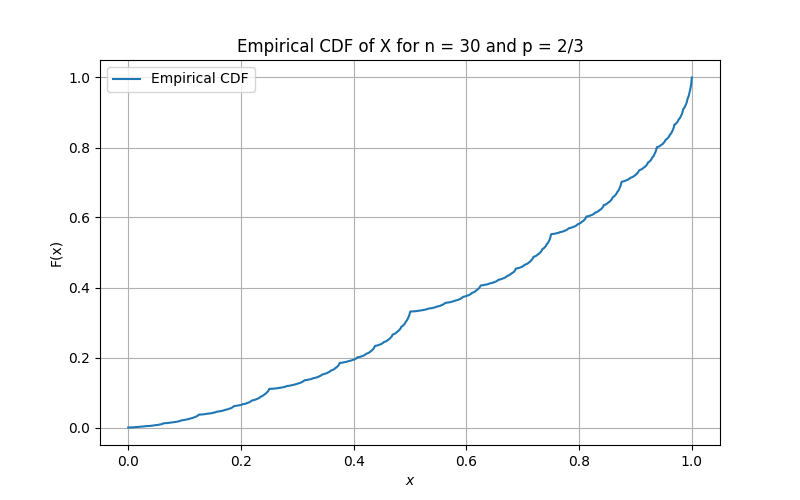
\includegraphics[width=1.0\linewidth]{images/empirical.png}
    \caption{\(N = 10000\)}
\end{figure}

\section{Exact Values of the CDF}

For some values of \(x\), the cumulative distribution function \(F(x) = \Pr(X \leq x)\) can be explicitly computed. In particular, let 
\[x = \sum_{i=1}^n \frac{x_i}{2^i}, \]
for fixed \(n \in \mathbf{N}\) and a sequence \(x_1, \dots, x_n \in \{0,1\}\). That is, \(x\) has a finite binary expansion. We need to find the probability that the random infinite binary expansion of \(X\) is less than or equal to the finite binary expansion of \(x\). This can be done by comparing digit by digit which we do recursively. Let us write the binary representations \(x = [0 \cdot x_1 \dots x_n]_2\) and \(X = [0 \cdot U_1 \dots]_2\).

We first note that \(x\) admits two binary representations if \(x > 0\) and \(x_n = 1\), namely \(x = [0 \cdot x_1 \dots x_{n-1}1000\dots]_2\) and \(x = [0 \cdot x_1 \dots x_n0111\dots]_2\), (the second expansion is not valid for \(x_n = 0\)). Let \(s = [0s_1, \dots s_n000\dots]_2\) be one binary expansion for \(x\). The event \(X = x\) via this sequence means \(U_i = s_i\) for all \(i\). The probability is then
\[ \Pr(X = x) = \prod_{i=1}^\infty \Pr(U_i = s_i) = \lim_{N \to \infty} (1-p)^{N-n} \prod_{i=1}^n \Pr(U_i = s_i) = 0, \]
and the same equality holds for the other binary expansion. Therefore \(F(x) = \Pr(X < x)\).

For \(x = [0.x_1 \dots x_n]_2\), consider the first coin toss \(U_1\):
\begin{enumerate}
    \item If \(U_1 < x_1\), then \(U_1 = 0\) and \(x_1 = 0\) so \(X \leq 1/2\) whilst \(x \geq 1/2\), so \(X < x\) is always true and we have \(\Pr(X < x \vert U_1 < x_1) = (1-p)x_1\).
    \item If \(U_1 > x_1\), then \(X < x\) is always false hence, \(\Pr(X < x | U_1 > x_1) = 0\).
    \item If \(U_1 = x_1\), then the condition \(X < x\) now fall to the next digits \(U_2\) and \(x_2\). We have the Bernoulli mass function \(\Pr(U_1 = x_1) = p^{x_1}(1-p)^{1-x_1}\), yielding the recursion
    \[ \Pr(X < x | U_1 = x_1) = p^{x_1}(1-p)^{1-x_1}F([0 \cdot 0x_2 \dots x_n]_2). \]
\end{enumerate}
Altogether, summing the conditional probabilities we obtain
\[ F(x) = x_1(1-p) + p^{x_1}(1-p)^{1-x_1}F([0 \cdot 0x_2 \dots x_n]_2). \]
Let \(x^{(k)} = [0 \cdot 0x_k \dots x_n]_2\) and \(P_j = p^{x_j}(1-p)^{1-x_j}\). We solve the recurrence
\[ F(x^{(k)}) = x_k(1-p) + P_kF(x^{(k+1)}) \]
by backwards iteration on \(k\). The base case \(k = n+1\) is trivial \(F(0) = F(X = 0) = 0\), so
\[ F(x^{(n)}) = x_n(1-p) + P_n\cdot 0 = x_n(1-p), \]
and continuing the backwards substitution yield
\[ F(x^{(1)}) = x_1(1-p) + x_2(1-p)P_1 + \dots + x_n(1-p)P_1 \dots P_n = \sum_{k=1}^n x_k(1-p)\prod_{j=1}^{k-1} P_j, \]
where the empty product is \(1\). Hence, we have
\[ F(x) = \sum_{k=1}^n x_k(1-p)\prod_{j=1}^{k-1} p^{x_j}(1-p)^{1-x_j}, \]
is the desired formula for the cumulative distribution function. We implement this algorithm below in a similar fashion to the empirical distribution function:

\begin{minted}[autogobble, linenos]{python}
    def binary_sequences(n):
    return np.array([
        [(i >> (n - j - 1)) & 1 for j in range(n)] 
    for i in range(2**n)])

    def F(p, sequence):
        F_x = 0
        for k in range(len(sequence)):
            if sequence[k] == 1:
                product = 1
                for j in range(k):
                    if sequence[j] == 1:
                        product *= p
                    else:
                        product *= (1 - p)
                F_x += (1 - p) * product
        return F_x
    
    def cdf(n, p):
        sequences = binary_sequences(n)
        x_values = np.linspace(0, 1, 2**n + 1)
        y_values = np.array([F(p, seq) for seq in sequences] + [1.0])
        return x_values, y_values
\end{minted}

For the empirical distribution, the time-complexity is \(O(Nn)\) provided the number of \(x\) values we test is dominated by the sample size \(N\). This is because generating the sample runs in \(O(Nn)\) time as it generates \(N\) sequences of length \(n\), whilst computing \(\hat{F}\) for \(N\) samples at \(M\) test points has time \(O(NM)\). This could potentially be improved by sorting the sample once \(O(N\log N\), then using binary search to compute at \(x\) the value of the CDF \(O(M\log N)\).

\begin{minted}[autogobble, linenos]{python}
    def ecdf(n, p, N):
        sample = generate_sample(n, p, N)
        sorted_sample = np.sort(sample)
        x_values = np.linspace(0, 1, 2**n + 1)
        y_values = np.searchsorted(sorted_sample, x_values, side='right') / N
        return x_values, y_values
\end{minted}

\begin{figure}
    \centering
    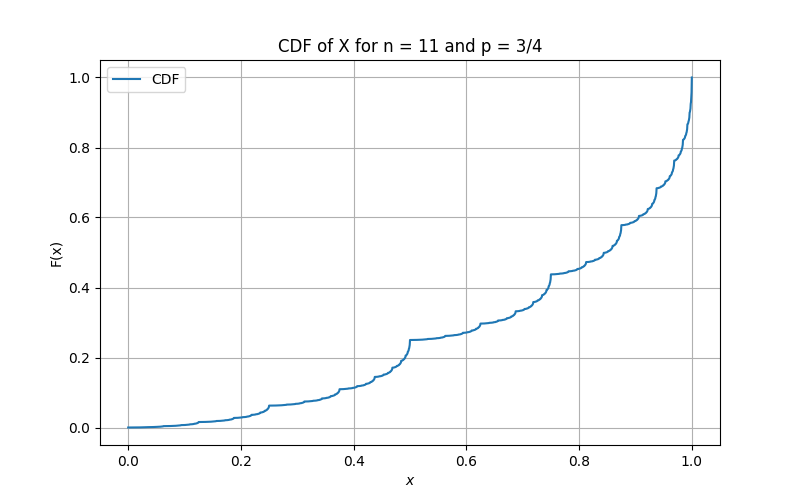
\includegraphics[width=1.0\linewidth]{images/truecdf.png}
    \caption{True CDF for \(X\), estimated at the dyadic rationals.}
\end{figure}

However, the time-complexity of our cumulative distribution function algorithm is \(O(n^22^n)\). Generating the binary sequences requires \(O(n2^n)\) time, as we loop over \(2^n\) integers and perform \(n\) bitwise operations. Computing \(F\) in the worst case is \(O(n^2)\), as the double loop scales alike the triangle numbers, and it is called \(2^n\) times. We can make an improvement when computing \(F\) since the product can be updated iteratively for each \(k\)F, reducing time complexity to \(O(n)\). 

\begin{minted}[autogobble, linenos]{python}
    def F(p, sequence):
        F_x = 0
        product = 1
        for k in range(len(sequence)):
            if sequence[k] == 1:
                F_x += (1 - p) * product
            if sequence[k] == 1:
                product *= p
            else: 
                product *= 1 - p
        return F_x
\end{minted}

Nevertheless, for large \(n\), this algorithm becomes infeasible to use.

\begin{figure}
    \centering
    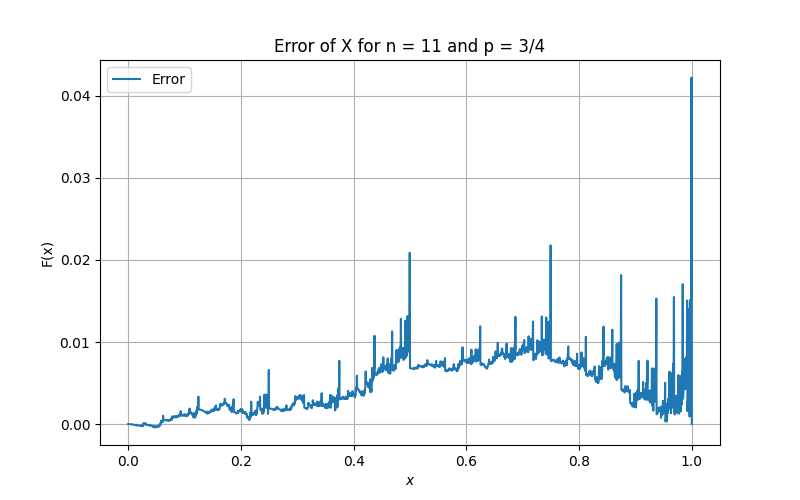
\includegraphics[width=1.0\linewidth]{images/error.png}
    \caption{The difference between the ECDF and CDF for \(X\).}
\end{figure}

Indeed, \(n = 11\) is quite small, but \(2^{11} = 2048\) is relatively computationally expensive.


\section{Properties of the CDF}

Recall that \(F\) is continuous at \(c\) if
\[ \lim_{x \to c^-} F(x) = F(c) = \lim_{x \to c^+} F(x). \]
Note that the right equality always holds for a valid CDF, so continuity is equivalent to the left equality. Since \(F(c) - \lim_{x \to c^-} F(x) = \Pr(X = c)\), we have that \(F(x)\) is continuous at \(c\) if and only if \(\Pr(X = c) = 0\).

Let \(c\) have a finite binary expansion. We first claim that \(F(x) = \Pr(X \leq x)\) is continuous at \(x = c\). Write \(X = [0 \cdot U_1 U_2\dots]_2\) and
\[ c = \frac{k}{2^n} = [0 \cdot c_1 \dots c_n]_2. \]
\begin{enumerate}
    \item If \(c = 0\), then 
    \[ \Pr(X = 0) = \Pr\left(\bigcap_{i=1}^\infty\{U_i = 0\}\right) = \prod_{i=1}^\infty \Pr(U_i = 0) = \prod_{i=1}^\infty (1 - p). \]
    Since \((1 - p) \in (0, 1)\), then \(\lim_{N \to \infty} (1 - p)^N = 0\) so \(\Pr(X = 0) = 0\).
    \item If \(c = 1\), then by symmetry, \(\lim_{N \to \infty} p^N = 0\), so \(\Pr(X = 1) = 0\).
    \item If \(c \in (0,1)\), then
    \[ \Pr(X = c) = \Pr\left(\bigcap_{i=1}^\infty\{U_i = c_i\}\right) = \prod_{i=1}^n \Pr(U_i = c_i)\prod_{i=n+1}^\infty \Pr(U_i = 0). \]
    The first term is finite, and the second term converges to \(0\) from above. Similarly, by considering the other binary representation of \(c\) we obtain \(\Pr(X = c) = 0\).
\end{enumerate}

From our previous plots, they seem to suggest that the cumulative distribution function is also continuous at all other points. Such points have infinite binary expansion \(c = [0 \cdot c_1c_2\dots]_2\), which must contain an infinite number of zeros or ones. Indeed, if the expansion is eventually constant, then it must be a dyadic rational number. Now,
\[ \Pr(X = c) = \Pr\left(\bigcap_{i=1}^\infty\{U_i = c_i\}\right) = \prod_{i=1}^\infty \Pr(U_i = c_i). \]
Define the partial product \(P_N = \prod_{i=1}^N \Pr(U_i = c_i) \). Each term \(\Pr(U_i = c_i)\) is either \(1 - p\) when \(c_i = 0\) or \(p\) when \(c_i = 1\). Let \(r = \max\{p,q\}\). Then
\[ 0 \leq P_n = \prod_{i=1}^N \Pr(U_i = c_i) \leq r^N \in (0,1), \]
so \(\lim_{N \to \infty} r^N = 0\) hence \(\lim_{N \to \infty} P_N = 0\) by the sandwich theorem. Therefore, we obtain \(\Pr(X = c) = 0\) as required. This means that the CDF \(F(x)\) is continuous on \([0,1]\).

Recall that \(F\) is left-differentiable at \(c\) if
\[ \lim_{\delta \to 0-} \frac{F(c + \delta) - F(c)}{\delta} \]
exists and is finite. Likewise, \(F\) is right-differentiable at \(c\) if
\[ \lim_{\delta \to 0+} \frac{F(c + \delta) - F(c)}{\delta}. \]
We say that \(F\) is differentiable at \(c\) if it is both left and right differentiable at \(c\). To estimate the difference quotients for dyadic rationals \(\delta\) in a neighbourhood of \(c\), we shall use the following code:

\begin{minted}[autogobble, linenos]{python}
    def difference_quotients(p, c, n):
        delta = 1 / (2 ** n)
        m_values = np.arange(-100, 100 + 1)
        m_values = m_values[m_values != 0]
        
        x_values = c + m_values * delta
        x_values = x_values[(x_values >= 0) & (x_values <= 1)]
        
        F_c = F(p, binary_expansion(c, n))
        F_x_values = np.array([F(p, binary_expansion(x, n)) for x in x_values])
        dq_values = (F_x_values - F_c) / (m_values * delta)
    
        return x_values, dq_values
\end{minted}

Set \(c = 9/16\) and \(p = 3/4\). We shall take \(\delta = 1 / 2^{11}\) as before to obtain a decent approximation of the derivative.

\begin{figure}
    \centering
    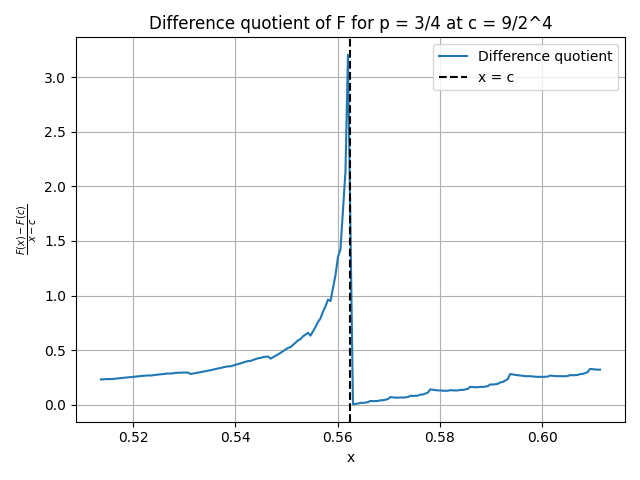
\includegraphics[width=0.45\linewidth]{images/derivative.png}
    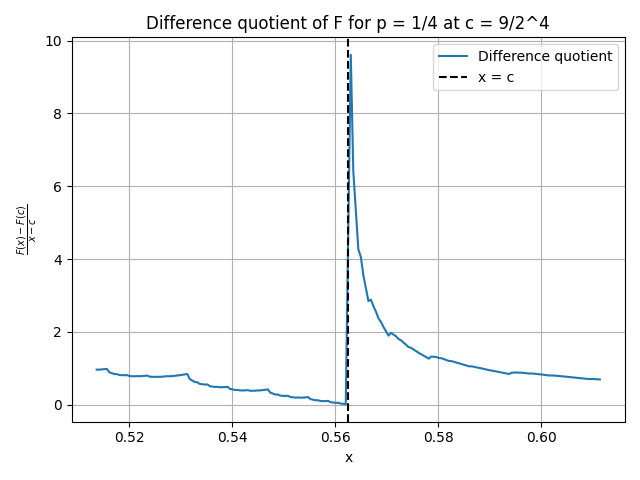
\includegraphics[width=0.45\linewidth]{images/derivative_2.png}
    \caption{Difference quotient in a neighbourhood of \(c = 9/16\).}
\end{figure}

From the plot, if \(p > 1/2\) then it seems that \(F\) is not left-differentiable at \(c\), since the difference quotient blows-up, whilst it is right-differentiable at \(c\) with vanishing derivative. The opposite happens for \(p < 1/2\). We conjecture the following result: At a dyadic rational point \(c\), \(F\) is left-differentiable at \(c\) if \(0 < p \leq 1/2\) and right-differentiable at \(c\) if \(1/2 \leq p < 0\).

Let \(\delta_L = \frac{1}{2^L}\) and write \(c = [0 \cdot c_1 \dots c_n]_2 \in [0,1]\) for \(L > n\).

\begin{itemize}
    \item Right-differentiability of \(c \in [0, 1)\): Consider the first expansion given by \(c = [0 \cdot c_1 \dots c_{n-1}1000 \dots]_2\). The interval \([c, c + \delta_L]\) consists of numbers whose binary expansions agree with that of \(c\) in the first \(n\) positions and are equal to \(0\) from position \(n+1\)  up to position \(L\). Therefore
    \[ \Pr(X \in [c, c+\delta_L]) = \prod_{i=1}^n \Pr(U_i = c_i) \prod_{i=n+1}^L \Pr(U_i = 0) = C_n (1-p)^{L-n}, \]
    where \(C_n := \prod_{i=1}^n \Pr(U_i = c_i)\). The difference quotient is now
    \[ \frac{C_n (1-p)^{L-n}}{\delta_L} = C_n (1-p)^{-n} (2(1-p))^L. \]
    Taking \(L \to \infty\), we see that this limit is finite if and only if \(p \leq 1/2\).
    
    \item Left-differentiability of \(c \in (0, 1]\): Consider the second expansion given by \(c = [0 \cdot c_1 \dots c_{n-1}0111 \dots]_2\). The interval \([c - \delta_L, c]\) consists of numbers whose binary expansions agree with that of \(c\) in the first \(n\) positions and are equal to \(1\) from position \(n+1\)  up to position \(L\). Therefore
    \[ \Pr(X \in [c - \delta_L, c]) = \prod_{i=1}^n \Pr(U_i = c_i) \prod_{i=n+1}^L \Pr(U_i = 0) = C_n p^{L-n}, \]
    where \(C_n := \prod_{i=1}^n \Pr(U_i = c_i)\). The difference quotient is now
    \[ \frac{C_n p^{L-n}}{\delta_L} = C_n p^{-n} (2p)^L. \]
    Taking \(L \to \infty\), we see that this limit is finite if and only if \(p \geq 1/2\).
\end{itemize}

To summarise, \(F\) is right-differentiable at a dyadic rational \(c \in [0,1)\) if and only if \(p \in (0, 1/2]\) with right-derivative \(1\) if \(p = 1/2\) and \(0\) otherwise. Likewise \(F\) is left-differentiable at a dyadic rational \(c \in (0,1]\) if and only if \(p \in [1/2, 1)\) with left-derivative \(1\) if \(p = 1/2\) and \(0\) otherwise. This also means that \(F\) is differentiable at \(c\) if and only if \(p = 1/2\).

\section{Monte Carlo Methods in Python}

NumPy in particular is very useful for Monte Carlo methods, owing to its probability distribution functions on arrays.

\end{document}
